

For the use of text-analyses, we read the paper "Probabilistic author-topic models for information discovery". This model is already used in the KDD-cup of 2013. The author-topic model creates a number of topics in which to classify the papers.  \cite{steyvers2004probabilistic}. The model not only discovers what topics are expressed in a document, but also which authors are associated with each topic. To simplify the representation of documents, the authors use a bag of words assumption that reduces each document to a vector of counts, where each vector element corresponds to the number of times a term appears in the document \cite{chowdhury2010introduction}. Each author is associated with a multinomial distribution over topics. A document with multiple authors has a distribution over topics that is a mixture of the distributions associated with the authors. When generating a document, an author is chosen at random for each individual word in the document. This author picks a topic from his or her multinomial distribution over topics, and then samples a word from the multinomial distribution over words associated with that topic. This process is repeated for all words in the document. In the model, the authors produce words from a set of $T$ topics. When $T$ is kept relatively small relative to the number of authors and vocabulary size, the author-topic model applies a form of dimensionality reduction to documents. Topics are learned which capture the variability in word choice across a large set of documents and authors. 

\begin{figure}
\begin{center}
	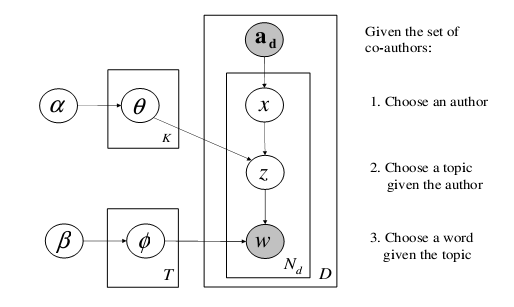
\includegraphics[scale=1]{./Images/model.png}
	\caption{The graphical model for the author-topic
model using plate notation.\cite{steyvers2004probabilistic} \label{fig:model}}
\end{center}
\end{figure}

Figure \ref{fig:model} illustrates the generative process with a graphical model using plate notation. In the author-topic model, observed variables not only include the words $w$ in a document but also the set of coauthors $A_d$ on each document $d$. Currently , the model does not specify the generative process of how authors choose to collaborate. Instead, the authors assume there is a co-author graph available. We create the graph in section \ref{sec:graph-background}